\section{Durchführung}
\label{sec:Durchführung}

Der Versuch wird gemäß \autoref{fig:Abb_3} aufgebaut.
\begin{figure}[H]
    \centering
    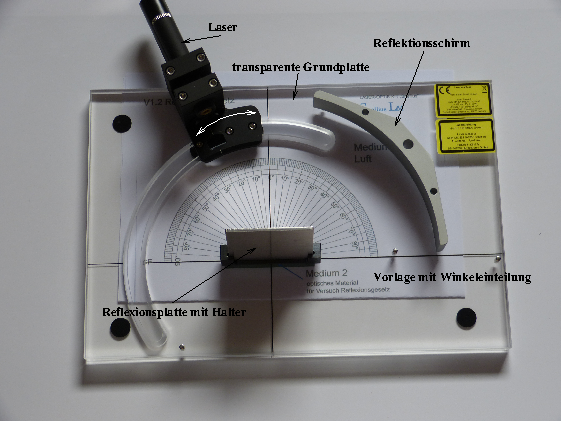
\includegraphics[width=0.8\textwidth]{build/Abb_3.pdf}
    \caption{Aufbau zur Messung des Photoeffektes.\cite{V500}}
    \label{fig:Abb_3}
\end{figure}
Das Licht der Spektrallampe fällt durch eine Kondensorlinse, einen Spalt und eine Abbildungslinse und wird 
somit gebündelt, bevor es das Prisma durchläuft.
Im Prisma wird der Lichtstrahl in Spektrallinien verschiedener Frequenzen gebrochen, welche auf die verschiebbare Photozelle treffen.\\
Nacheinander werden nun $5$ verschiedene Spektrallinien untersucht.
Hierbei wird darauf geachtet, die jeweilige Spektrallinie mithilfe der Linsen möglichst scharf zu fokussieren und den Spalt der
Photozelle darauf auszurichten.
Für $5$ verschiedene Linien wird der am Picoamperemeter gemessene Photostrom in Abhängigkeit von der angelegten Bremsspannung gemessen.
Hierbei wird die Bremsspannung erhöht, bis kein Photostrom mehr festzustellen ist.
Für die gelbe Linie wird zudem zusätzlich der Bereich bis ca. $\qty{20}{\volt}$ Beschleunigungsspannung gemessen.
Die Werte werden tabellarisch aufgenommen.
Zwischen den einzelnen Messungen muss das Bild eventuell erneut fokussiert werden.